\input{eng_boo.aaa}
\begin{document}
\entete{LFA} {Autodocumented Files Software} {Jean-Marcel Piriou, CNRM/GMAP} 
{\aujour, Version 2} 
{logo_lfa.ps}{height=11.cm,angle=-90.}

%%%%%%%%%%%%%%%%%%%%%%%%%%%%%%%%%%%%%%%%%%%%%%%%%%%%%%%%%%%%%%%%%%%%%%%%%
\chapter{Main features}

\pa  The present AFS software
(LFA in French, Logiciel de Fichiers Autodocument�s) is designed to 
read or write real, integer or character arrays, on portable
files (IEEE binairies), will a portable code.
Articles in the files are accessed through their name.

\p The underlying idea of this software is to combine two
abilities: firstly an access to a given article through its
name, for a simpler and more secured access to file data,
and secondly physical write on IEEE binaries to assure
execution speed and portability.

\p The user interface allows file handling
from fortran codes,
but also directly from UNIX system command line. 

\p One can 
open/close files, read/write articles, copy some
articles from one file
to another, fuse files, 
print out the list of articles in a file (with type of data, length,
name, extrema, ...), 
read a LFA article on standard output in text form,
create a LFA article from standard input in text form,
etc... This allows user to forget
some of "basic I/O notions" while using large variety of data.


\section*{Performance}

\pa One has controlled execution speed and file space for
writing and reading 150000 4 bytes real data on file, 
with three methods: unformatted, LFA and formatted.

\p Time are given in seconds
on a HP-UX 9000/715 station, size in bytes.

\p \begin{tabular}{|l|r|r|}\hline 
	Software & Size & Execution time \\ \hline
	unformatted & 600008 & 0.1 \\
	LFA & 600056 & 0.2 \\
	formatted & 2550000 & 15.5 \\
	\hline
\end{tabular}

\p Unformatted I/O is very rapid, since it is a simple
copy from memory to disk: unformatted I/O is  100 times quicker
than formatted I/O!...

\section*{Data precision}

\pa LFA software is designed to read/write 4 and 8 bytes
integer and real data. A library is provided by the install
script, per precision. By precision we stand here for precision 
of dummy arguments given by user to fortran LFA routines.
The library names are explicit, for example
{\tt liblfa\_R8I4.a} for a library to be use by a program giving
8 bytes real and 4 bytes integer data as arguments to LFA.

\p However, even if you have choosen a given user precision
for dummy arguments, you are not required to write/read on files
at that precision:
you can write in file 4 bytes precision
data calculated on 8 bytes (in order to save disk space),
or read on array at user precision X
data at Y precision on file. The LFA software
make the interface between file and user precision
in a transparent way.

\p If no explicit precision is given by you, the default
is to write at user dummy arguments precision.
This write precision can be changed before each article
write, and thus it is possible to write in the same
file data from different precisions (see lfaprecr and lfapreci).

\section*{File portability}

\pa File will be portable between machines having
the same internal data representation. 
Many machines follow presently the IEEE format,
and thus portability inside this familiy will
be possible.

\p CRAY case: this machine is not IEEE, but
can produce IEEE binairies, through the
"assign -N ieee" command; this command has been
used under "\#ifdef cray" key
in the LFA software, to produce IEEE
format files even on CRAY.

\section*{Synoptic of main functions}

\centerline{
\includegraphics
	[angle=-90, 
	width=12.cm, 
	keepaspectratio=true,
	clip=true]
	{organigramme.ag.eps}
}

\pa The LFA utilities from the present documentation have
been put in the above diagram: the interface between 
a LFA file and computer core memory is done
by fortran routines lfalec* (read) and lfaecr* (write).

\p The LFA utilities to be called DIRECTLY from UNIX
command line are in red: get the list of file articles,
modify a LFA file with your usual text editor, extract
a given article on standard output, make the difference
between two LFA files, etc... These operations
can be managed without any user fortran coding.

%%%%%%%%%%%%%%%%%%%%%%%%%%%%%%%%%%%%%%%%%%%%%%%%%%%%%%%%%%%%%%%%%%%%%%%%%
\chapter{Fortran user interface}

\pa One describes here the fortran user interface,
that is the routines that user wiil call from its own
codes to read, write or deal in general with LFA files.


\section{lfaouv: Open}
 
 
 
\begin{verbatim}
	subroutine lfaouv(kul,cdnomf,cdtypo)
	! -------------------------------------------------------------                
	! **** *LFAOUV* Ouverture de fichier LFA.
	! -------------------------------------------------------------                
	! **** *LFAOUV* Open a LFA file.
	! -------------------------------------------------------------                
	! En entree:
	! kul         unite logique du fichier.
	! cdnomf      nom du fichier.
	! cdtypo      type d'ouverture: 'R' READ, 'W' WRITE, 'A' APPEND, 'S' SCRATCH.
	! En sortie:
	! --------------------------------------------------------------------------
	! Input:
	! kul         logical unit of LFA file.
	! cdnomf      file name.
	! cdtypo      opening type: 'R' READ, 'W' WRITE, 'A' APPEND, 'S' SCRATCH.
	! Output:
	! --------------------------------------------------------------------------
\end{verbatim}
\section{lfafer: Close}
 
 
 
\begin{verbatim}
	subroutine lfafer(kul)
	! -------------------------------------------------------------                
	! **** *LFAFER* Fermeture de fichier LFA.
	! -------------------------------------------------------------                
	! **** *LFAFER* Close a LFA file.
	! -------------------------------------------------------------                
	! En entree:
	! kul        unite logique du fichier.
	! En sortie:
	! --------------------------------------------------------------------------
	! Input:
	! kul        logical unit of LFA file.
	! Output:
	! --------------------------------------------------------------------------
\end{verbatim}
 
\section{lfaprecr: Force real data writing precision}
 
 
\begin{verbatim}
	subroutine lfaprecr(kul,kprec)
	! -------------------------------------------------------------                
	! **** *LFAPRECR* Forcage de la precision d'ecriture des reels.
	! -------------------------------------------------------------                
	! **** *LFAPRECR* Force real data writing precision.
	! -------------------------------------------------------------                
	! En entree:
	! kul      unite logique du fichier LFA.
	! kprec    precision des reels a ecrire ulterieurement, en octets.
	! En sortie:
	! --------------------------------------------------------------
	! Input:
	! kul      logical unit of LFA file.
	! kprec    precision of real data to write, in bytes.
	! Output:
	! --------------------------------------------------------------
\end{verbatim}
 
\section{lfapreci: Force integer data writing precision}
\begin{verbatim}
	subroutine lfapreci(kul,kprec)
	! -------------------------------------------------------------                
	! **** *LFAPRECI* Forcage de la precision d'ecriture des entiers.
	! -------------------------------------------------------------                
	! **** *LFAPRECI* Force integer data writing precision.
	! -------------------------------------------------------------                
	! En entree:
	! kul      unite logique du fichier LFA.
	! kprec    precision des entiers a ecrire ulterieurement, en octets.
	! En sortie:
	! --------------------------------------------------------------
	! Input:
	! kul      logical unit of LFA file.
	! kprec    precision of integer data to write, in bytes.
	! Output:
	! --------------------------------------------------------------
\end{verbatim}

\section{lfaecrr: Write real data }
 
 
 
\begin{verbatim}
	subroutine lfaecrr(kul,cdna,preel,klong)
	! -------------------------------------------------------------                
	! **** *LFAECRR* Ecriture de reels sur fichier LFA.
	! -------------------------------------------------------------                
	! **** *LFAECRR* Write real data on LFA file.
	! -------------------------------------------------------------                
	! En entree:
	! kul              unite logique du fichier.
	! cdna             nom de l'article a ecrire.
	! preel(1,klong)   reels a ecrire.
	! klong            longueur de l'article a ecrire.
	! En sortie:
	! --------------------------------------------------------------------------
	! Input:
	! kul              logical unit of LFA file.
	! cdna             name of article to write.
	! preel(1,klong)   real data to write.
	! klong            length of article to write.
	! Output:
	! --------------------------------------------------------------------------
\end{verbatim}
\section{lfaecri: Write integer data }
 
 
 
\begin{verbatim}
	subroutine lfaecri(kul,cdna,kentier,klong)
	! -------------------------------------------------------------                
	! **** *LFAECRI* Ecriture d'entiers sur fichier LFA.
	! -------------------------------------------------------------                
	! **** *LFAECRI* Write integer data of LFA file.
	! -------------------------------------------------------------                
	! En entree:
	! kul                  unite logique du fichier.
	! cdna                  nom de l'article a ecrire.
	! kentier(1,klong)      entiers a ecrire.
	! klong            longueur de l'article a ecrire.
	! En sortie:
	! --------------------------------------------------------------------------
	! Input:
	! kul                  logical unit of LFA file.
	! cdna                 name of article to write.
	! kentier(1,klong)     integers to write.
	! klong                length of article to write.
	! Output:
	! --------------------------------------------------------------------------
\end{verbatim}
\section{lfaecrc: Write character data }
\begin{verbatim}
	subroutine lfaecrc(kul,cdna,cdcar,klong)
	! -------------------------------------------------------------                
	! **** *LFAECRC* Ecriture de caracteres sur fichier LFA.
	! -------------------------------------------------------------                
	! **** *LFAECRC* Write character data on LFA file.
	! -------------------------------------------------------------                
	! En entree:
	! kul              unite logique du fichier.
	! cdna             nom de l'article a ecrire.
	! cdcar(1,klong)   caracteres a ecrire.
	! klong            longueur de l'article a ecrire.
	! En sortie:
	! --------------------------------------------------------------------------
	! Input:
	! kul              logical unit of LFA file.
	! cdna             name of article to write.
	! cdcar(1,klong)   characters to write.
	! klong            length of article to write.
	! Output:
	! --------------------------------------------------------------------------
\end{verbatim}
\section{lfalecr: Read real data }
 
 
 
\begin{verbatim}
	subroutine lfalecr(kul,cdna,kdimb,preel,klong,kerr)
	! -------------------------------------------------------------                
	! **** *LFALECR* Lecture de reels sur fichier LFA.
	! -------------------------------------------------------------                
	! **** *LFALECR* Read real data on LFA file.
	! -------------------------------------------------------------                
	! En entree:
	! kul              unite logique du fichier.
	! cdna             nom de l'article.
	! kdimb            dimension du tableau preel.
	! En sortie:
	! klong            nombre de reels lus.
	! preel(1,klong)   reels lus.
	! kerr             indicateur d'erreur:
	! +----------+-----------------------------------------------------+
	! | Valeur   |             Signification                           |
	! +----------+-----------------------------------------------------+
	! | kerr=  0 | Tout est OK!                                        |
	! | kerr= -1 | Article inexistant                                  |
	! | kerr= -6 | Article plus long que le tableau devant le recevoir |
	! | kerr= -8 | Mauvais type de donnees (reelles, entieres, car.)   |
	! +----------+-----------------------------------------------------+
	! --------------------------------------------------------------------------
	! Input:
	! kul              logical unit of LFA file.
	! cdna             article name.
	! kdimb            physical dimension of array preel.
	! Output:
	! klong            number of real elements read.
	! preel(1,klong)   real elements read.
	! kerr             error indicator:
	! +----------+-----------------------------------------------------+
	! | Value    |             Meaning                                 |
	! +----------+-----------------------------------------------------+
	! | kerr=  0 | Everything is OK!                                   |
	! | kerr= -1 | Article inexistant                                  |
	! | kerr= -6 | Article bigger than array supposed to receive it    |
	! | kerr= -8 | Wrong data type (real, integer, char.)              |
	! +----------+-----------------------------------------------------+
	! --------------------------------------------------------------------------
\end{verbatim}
\section{lfaleci: Read integer data }
 
 
 
\begin{verbatim}
	subroutine lfaleci(kul,cdna,kdimb,kentier,klong,kerr)
	! -------------------------------------------------------------                
	! **** *LFALECI* Lecture d'entiers sur fichier LFA.
	! -------------------------------------------------------------                
	! **** *LFALECI* Read integer data on LFA file.
	! -------------------------------------------------------------                
	! En entree:
	! kul              unite logique du fichier.
	! cdna             nom de l'article.
	! kdimb            dimension du tableau kentier.
	! En sortie:
	! klong            nombre d'entiers lus.
	! kentier(1,klong) entiers lus.
	! kerr             indicateur d'erreur:
	! +----------+-----------------------------------------------------+
	! | Valeur   |             Signification                           |
	! +----------+-----------------------------------------------------+
	! | kerr=  0 | Tout est OK!                                        |
	! | kerr= -1 | Article inexistant                                  |
	! | kerr= -6 | Article plus long que le tableau devant le recevoir |
	! | kerr= -8 | Mauvais type de donnees (reelles, entieres, car.)   |
	! +----------+-----------------------------------------------------+
	! --------------------------------------------------------------------------
	! Input:
	! kul              logical unit of LFA file.
	! cdna             article name.
	! kdimb            physical dimension of array kentier.
	! Output:
	! klong            number of integer elements read.
	! kentier(1,klong) integer elements read.
	! kerr             error indicator:
	! +----------+-----------------------------------------------------+
	! | Value    |             Meaning                                 |
	! +----------+-----------------------------------------------------+
	! | kerr=  0 | Everything is OK!                                   |
	! | kerr= -1 | Article inexistant                                  |
	! | kerr= -6 | Article bigger than array supposed to receive it    |
	! | kerr= -8 | Wrong data type (real, integer, char.)              |
	! +----------+-----------------------------------------------------+
	! --------------------------------------------------------------------------
\end{verbatim}
\section{lfalecc: Read character data }
 
 
\begin{verbatim}
	subroutine lfalecc(kul,cdna,kdimb,cdcar,klong,kerr)
	! -------------------------------------------------------------                
	! **** *LFALECC* Lecture de caracteres sur fichier LFA.
	! -------------------------------------------------------------                
	! **** *LFALECC* Read character data on LFA file.
	! -------------------------------------------------------------                
	! En entree:
	! kul              unite logique du fichier.
	! cdna             nom de l'article.
	! kdimb            dimension du tableau cdcar.
	! En sortie:
	! klong            nombre de chaines de caracteres lues.
	! cdcar(1,klong)   chaines lues.
	! kerr             indicateur d'erreur:
	! +----------+-----------------------------------------------------+
	! | Valeur   |             Signification                           |
	! +----------+-----------------------------------------------------+
	! | kerr=  0 | Tout est OK!                                        |
	! | kerr= -1 | Article inexistant                                  |
	! | kerr= -6 | Article plus long que le tableau devant le recevoir |
	! | kerr= -8 | Mauvais type de donnees (reelles, entieres, car.)   |
	! +----------+-----------------------------------------------------+
	! --------------------------------------------------------------------------
	! Input:
	! kul              logical unit of LFA file.
	! cdna             article name.
	! kdimb            physical dimension of array cdcar.
	! Output:
	! klong            number of character elements read.
	! cdcar(1,klong)   character elements read.
	! kerr             error indicator:
	! +----------+-----------------------------------------------------+
	! | Value    |             Meaning                                 |
	! +----------+-----------------------------------------------------+
	! | kerr=  0 | Everything is OK!                                   |
	! | kerr= -1 | Article inexistant                                  |
	! | kerr= -6 | Article bigger than array supposed to receive it    |
	! | kerr= -8 | Wrong data type (real, integer, char.)              |
	! +----------+-----------------------------------------------------+
	! --------------------------------------------------------------------------
\end{verbatim}
\section{lfatest: Test if a file is a LFA one}
 
 
 
\begin{verbatim}
	subroutine lfatest(kul,cdnomf,ldlfa)
	! -------------------------------------------------------------                
	! **** *LFATEST* Teste si un fichier est bien de type LFA.
	! -------------------------------------------------------------                
	! **** *LFATEST* Test if a file is a LFA one.
	! -------------------------------------------------------------                
	! En entree:
	! kul         unite logique du fichier;
	! .           ce doit etre une unite disponible:
	! .           le fichier va etre ouvert sous cette unite logique.
	! cdnomf      nom du fichier.
	! En sortie:
	! ldlfa=.true. si le fichier est de type LFA, .false. sinon.
	! --------------------------------------------------------------------------
	! Input:
	! kul         logical unit of file.
	! .           this unit has to be free:
	! .           the file will be opened with this logical unit.
	! cdnomf      file name.
	! Output:
	! ldlfa=.true. if the file is a LFA one, .false. else case.
	! --------------------------------------------------------------------------
\end{verbatim}
 
\section{lfames: Print out level of software}
 
 
 
\begin{verbatim}
	subroutine lfames(kul,kmes)
	! -------------------------------------------------------------                
	! **** *LFAMES* Niveau de messagerie du logiciel LFA.
	! -------------------------------------------------------------                
	! **** *LFAMES* Print out level of LFA software.
	! -------------------------------------------------------------                
	! En entree:
	! kul         unite logique du fichier.
	! kmes        niveau de messagerie:
	! si 0 aucun message sorti par le logiciel LFA.
	! si 1 messages d'ATTENTION et d'ERREUR sorties.
	! si 2 LFA est bavard (a reserver au debug de LFA...).
	! En sortie:
	! --------------------------------------------------------------------------
	! Input:
	! kul         logical unit of LFA file.
	! kmes        print out level:
	! if 0 no message print out.
	! if 1 WARNING or ERROR messages print out.
	! if 2 many comments print out (LFA debug mode only...).
	! Output:
	! --------------------------------------------------------------------------
\end{verbatim}
 
\section{lfaerf: Choose error level of software}
 
 
 
\begin{verbatim}
	subroutine lfaerf(kul,lderf)
	! -------------------------------------------------------------                
	! **** *LFAERF* Niveau d'erreur tolere par le logiciel LFA.
	! -------------------------------------------------------------                
	! **** *LFAERF* Choose error level of LFA software.
	! -------------------------------------------------------------                
	! En entree:
	! kul               unite logique du fichier.
	! lderf             .true. si toute erreur doit etre fatale,
	! .false. si aucune ne doit l'etre.
	! En sortie:
	! lgerf             .true. si toute erreur est fatale,
	! .false. si aucune ne l'est.
	! --------------------------------------------------------------------------
	! Input:
	! kul               logical unit of LFA file.
	! lderf             .true. if any error has to be fatal.
	! .false. si none has to be.
	! Output:
	! lgerf             .true. if any error has to be fatal.
	! .false. si none has to be.
	! --------------------------------------------------------------------------
\end{verbatim}
\section{lfalaf: Article list}
 
 
 
\begin{verbatim}
	subroutine lfalaf(kul,kulout)
	! -------------------------------------------------------------                
	! **** *LFALAF* Liste des articles d'un fichier LFA.
	! -------------------------------------------------------------                
	! **** *LFALAF* Article list of a LFA file.
	! -------------------------------------------------------------                
	! En entree:
	! kul             unite logique du fichier.
	! kulout          unite logique sur laquelle sortir la liste.
	! En sortie:
	! --------------------------------------------------------------------------
	! Input:
	! kul             logical unit of LFA file.
	! kulout          logical unit on which print out the list.
	! Output:
	! --------------------------------------------------------------------------
\end{verbatim}
\section{lfalaft: Article list, on an array}
 
 
 
\begin{verbatim}
	subroutine lfalaft(kul,cdlis,kdlis,knlis)
	! -------------------------------------------------------------                
	! **** *LFALAFT* Liste des articles d'un fichier LFA sur tableau de caracteres.
	! -------------------------------------------------------------                
	! **** *LFALAFT* Article list of a LFA file, on an array.
	! -------------------------------------------------------------                
	! En entree:
	! kul             unite logique du fichier.
	! kdlis           dimension physique du tableau cdlis.
	! En sortie:
	! knlis           nombre d'articles du fichier.
	!                 Ce nombre est egalement le nombre d'elements ecrits sur cdlis
	! cdlis(1, ..., knlis) nom des articles du fichier.
	! --------------------------------------------------------------------------
	! Input:
	! kul            logical unit of LFA file.
	! kdlis          physical dimension of array cdlis.
	! Output:
	! knlis          number of articles on the file.
	!                This number is also the number of elements written on cdlis.
	! cdlis(1, ..., knlis) article names.
	! --------------------------------------------------------------------------
\end{verbatim}
 
\section{lfaminm: Extrema of all articles}
 
 
\begin{verbatim}
	subroutine lfaminm(kul)
	! -------------------------------------------------------------                
	! **** *LFAMINM* Extrema de tous les articles d'un fichier LFA.
	! -------------------------------------------------------------                
	! **** *LFAMINM* Extrema of all articles of a given LFA file.
	! -------------------------------------------------------------                
	! En entree:
	! kul unite logique du fichier LFA d'entree.
	! En sortie:
	! Extrema sur output standard.
	! --------------------------------------------------------------
	! Input:
	! kul logical unit of LFA file.
	! Output:
	! Extrema on standard output.
	! --------------------------------------------------------------
\end{verbatim}

\section{lfacas: Get documentation about an article}
\begin{verbatim}
	subroutine lfacas(kul,cdna,cdtype,klong,kerr)
	! -------------------------------------------------------------                
	! **** *LFACAS* Renseignements sur un article de fichier LFA.
	! -------------------------------------------------------------                
	! **** *LFACAS* Get documentation about a LFA article.
	! -------------------------------------------------------------                
	! En entree:
	! kul               unite logique du fichier.
	! cdna: si cdna=' ' on recherche l'article suivant.
	! .         cdna est alors en entree/sortie,
	! .         et en sortie il vaudra le nom de l'article suivant
	! .         (si cet article existe).
	! .         kerr...retour de recherche: 0 si OK,
	! .                1 si fin de fichier.
	! .     si cdna<>' ' cdna est le nom de l'article cherche.
	! .          Il est alors en entree seulement.
	! .         kerr...retour de recherche: 0 si OK,
	! .                1 si article inexistant.
	! En sortie:
	! cdtype            type d'article: 'R4', 'I8', 'C '.
	! klong             nombre d'elements de cet article.
	! --------------------------------------------------------------------------
	! Input:
	! kul               file logical unit.
	! cdna: if cdna=' ' on looks for nbext article.
	! .         cdna is then in input/output
	! .         and in output it will receive next article name
	! .         (if this article exists).
	! .         kerr...return from search: 0 if OK,
	! .                1 if end of file.
	! .     if cdna<>' ' cdna is the name from required article.
	! .          It is then in input olny.
	! .         kerr...return from search: 0 if OK,
	! .                1 if non-existant article.
	! Output:
	! cdtype            article type: 'R4', 'I8', 'C '.
	! klong             numbre of elements in this article.
	! --------------------------------------------------------------------------
\end{verbatim}

\section{lfaavan: Step over current article}
 
 
\begin{verbatim}
	subroutine lfaavan(kul)
	! -------------------------------------------------------------                
	! **** *LFAAVAN* Saute l'article courant dans un fichier LFA.
	! -------------------------------------------------------------                
	! **** *LFAAVAN* Step over current article in an LFA file.
	! -------------------------------------------------------------                
	! En entree:
	! kul               unite logique du fichier.
	! En sortie:
	! --------------------------------------------------------------------------
	! Input:
	! kul               logical unit of the LFA file.
	! Output:
	! --------------------------------------------------------------------------
\end{verbatim}

\section{lfarew: Rewind}

\pa Cet appel sert dans le cas rare suivant: vous avez lu
certains articles du fichier, puis vous voulez lire tous les articles
du fichier s�quentiellement via lfacas. lfacas fournissant 
le nom de l'article suivant, il faut au pr�alable rebobiner
le fichier par lfarew.

\p Ce cas est rare: en g�n�ral, soit on lit des articles en y acc�dant
directement par leur nom, auquel cas la gestion
du pointeur fichier est effectu�e de fa�on 
transparente par le logiciel LFA, soit on veut lire tout le fichier
s�quentiellement, et on le fait d�s son ouverture,  et il
n'y a donc pas lieu de rebobiner!... 
 
 
 
\begin{verbatim}
	subroutine lfarew(kul)
	! -------------------------------------------------------------                
	! **** *LFAREW* Rebobinage d'un fichier LFA.
	! -------------------------------------------------------------                
	! **** *LFAREW* Rewind a LFA file.
	! -------------------------------------------------------------                
	! En entree:
	! kul: unite logique du fichier LFA.
	! En sortie:
	! --------------------------------------------------------------
	! Input:
	! kul: logical unit of LFA file.
	! En sortie:
	! --------------------------------------------------------------
\end{verbatim}

\section{lfacop: Copy one article from a LFA file to another}
\begin{verbatim}
	subroutine lfacop(kule,cdnae,cdnas,kuls)
	! -------------------------------------------------------------                
	! **** *LFACOP* Copie d'un article d'un fichier LFA a un autre.
	! -------------------------------------------------------------                
	! **** *LFACOP* Copy one article from a LFA file to another.
	! -------------------------------------------------------------                
	! En entree:
	! kule unite logique du fichier LFA d'entree.
	! cdnae nom de l'article a lire.
	! cdnas nom sous lequel l'article est recopie.
	! kuls unite logique du fichier LFA de sortie.
	! En sortie:
	! Le fichier d'unite logique kuls est augmente d'un article.
	! --------------------------------------------------------------
	! Input:
	! kule logical unit of input LFA file.
	! cdnae article name to be read.
	! cdnas article name to be written out.
	! kuls logical unit of output LFA file.
	! Output:
	! The file which logical unit is kuls receives one more article.
	! --------------------------------------------------------------
\end{verbatim}
%%%%%%%%%%%%%%%%%%%%%%%%%%%%%%%%%%%%%%%%%%%%%%%%%%%%%%%%%%%%%%%%%%%%%%%%%
\chapter{UNIX user interface}

\pa LFA files can contain various data,
and thus it is very often useful to access to information
from LFA files directly from the UNIX command line:
get the list of all articles in a LFA file, which are
the extrema of data in these articles, create a LFA file
directly from ASCII text files, etc...
The sources from such utilities are proposed
with the LFA package, and their executable version
is created by default install process.

\p The synopsis and usage of these utilities are proposed
below. They can also be obtained from command line: type
a LFA command with no argument will give you 
the sysnopsis and usage on standard output.

%%%%%%%%%%%%%%%%%%%%%%%%%%%%%%%%%%%%%%%%%%%%%%%%%%%%%%%%%%%%%%%%%%%%%%%%%
\section{lfalaf: Get the articles list of a LFA file}
\begin{verbatim}
  
 Get the articles list of a LFA file.
  
 Usage: lfalaf FILE
  

\end{verbatim}

%%%%%%%%%%%%%%%%%%%%%%%%%%%%%%%%%%%%%%%%%%%%%%%%%%%%%%%%%%%%%%%%%%%%%%%%%
\section{lfaminm: Prints out extrema of all articles}
\begin{verbatim}
 
Prints out extrema, mean and rms of all articles from one (or more) LFA file(s).
 
Usage: lfaminm LFA1 [LFA2 ... LFAn]
 

\end{verbatim}

%%%%%%%%%%%%%%%%%%%%%%%%%%%%%%%%%%%%%%%%%%%%%%%%%%%%%%%%%%%%%%%%%%%%%%%%%
\section{lfaedit: Edit one (or more) LFA file(s)}
\begin{verbatim}
 
Edit one (or more) LFA file(s).
The goal is here to visualize or modify 
a LFA file directly with your usual editor.
 
Usage: lfaedit F1 [F2 ... Fn]
 
Principle: files are transformed into the LFP form (ASCII text),
then one calls the editor. Files in output from editor,
if modified, are transformed back to the LFA form.
The invoked editor is given by EDITOR environment variable.
 

\end{verbatim}

%%%%%%%%%%%%%%%%%%%%%%%%%%%%%%%%%%%%%%%%%%%%%%%%%%%%%%%%%%%%%%%%%%%%%%%%%
\section{lfac: Extract one article on standard output }
\begin{verbatim}
  
 Extract on standard output one LFA article.
  
 Usage: lfac FILE ARTICLE
 with
     FILE: LFA file name.
     ARTICLE: article name in the file.
  

\end{verbatim}

%%%%%%%%%%%%%%%%%%%%%%%%%%%%%%%%%%%%%%%%%%%%%%%%%%%%%%%%%%%%%%%%%%%%%%%%%
\section{lfacop: copy articles from a file to another}
\begin{verbatim}
   
 Copy n articles from a LFA file to another LFA file.
   
 Usage: lfac LFA1 LFA2 ART1 [ART2 ... ARTn]
 with
     LFA1: input LFA file.
     LFA2: output LFA file.
     ART1 [ART2 ... ARTn]: articles list.
   
  
\end{verbatim}

%%%%%%%%%%%%%%%%%%%%%%%%%%%%%%%%%%%%%%%%%%%%%%%%%%%%%%%%%%%%%%%%%%%%%%%%%
\section{lfareu: Fuse two LFA files}
\begin{verbatim}
  
 Fuse two LFA files.
  
 Usage: lfareu F1 F2 Fres
        In input: F1 and F2, in output: Fres.
        F2 has higher priority than F1, i.e. if an article
        is present in both F1 and F2, the article from F2 will be copied.
  

\end{verbatim}

%%%%%%%%%%%%%%%%%%%%%%%%%%%%%%%%%%%%%%%%%%%%%%%%%%%%%%%%%%%%%%%%%%%%%%%%%
\section{lfamoy: Mean of n files}
\begin{verbatim}
  
 Mean of n LFA files.
  
 Usage: lfamoy FMEA F1 F2 [F3 ... Fn]
 with
        F1 F2 [F3 ... Fn] the n input files.
        FMEA the output file, receiving mean value.
  
 Nota: the mean is performed on articles
 present in all files.
  
\end{verbatim}

%%%%%%%%%%%%%%%%%%%%%%%%%%%%%%%%%%%%%%%%%%%%%%%%%%%%%%%%%%%%%%%%%%%%%%%%%
\section{lfacre: Create a LFA file from command line}
\begin{verbatim}
 
Create a LFA file from command line
and(or) from ASCII text file(s).
 
Usage:
 
lfacre LFA [article_name_1 type_1 fil_name_1] ... [article_name_n type_n fil_name_n]
n has to be less than  20
In output, the LFA file will contain the n articles
article_name_1 to article_name_n, which type will be type_1 to type_n (type: R4, R8, I4, I8 ou C),
and contents of these articles will be fil_name_1 to fil_name_n:
        - If fil_name_i is a file, then its contents
          will be put in article_name_i article.
        - If fil_name_i is not a file, then it is the value
          of the one-value article article_name_i.
 
Example:
 
cat <<EOF > gol
gol1
gol2
EOF
lfacre LFA RII0 R 1370. indice C gol year I 2006
will create the file LFA, containing tree articles, the real data article RII0
(length 1), the character data article indice (length 2),
and the integer data article year (length 1).
 

\end{verbatim}

%%%%%%%%%%%%%%%%%%%%%%%%%%%%%%%%%%%%%%%%%%%%%%%%%%%%%%%%%%%%%%%%%%%%%%%%%
\section{lfadiff: Difference between two LFA files}
\begin{verbatim}
  
 Difference between two LFA files.
  
 Usage: lfadiff F1 F2 FDIFF
 with
        F1 and F2 the two input files.
        FDIFF the output LFA file, receiving F2-F1.
  
 Nota: the difference is calculated on articles
 present in both files.
  

\end{verbatim}

%%%%%%%%%%%%%%%%%%%%%%%%%%%%%%%%%%%%%%%%%%%%%%%%%%%%%%%%%%%%%%%%%%%%%%%%%
\section{lfadiffrel: Relative difference between two LFA files}
\begin{verbatim}
  
 Relative difference between two LFA files.
  
 Usage: lfadiffrel F1 F2 FDIFF
 with
        F1 and F2 the two input files.
        FDIFF the output file, receiving (F2-F1)/rms(F1).
  
 rms(F1) is the root mean squared of the F1 article.
 Nota: the difference is calculated on articles
  present in both files.
  
 If rms(F1)=0, result is 0 if F2=0, and equal to  999.999 else case.
  

\end{verbatim}

%%%%%%%%%%%%%%%%%%%%%%%%%%%%%%%%%%%%%%%%%%%%%%%%%%%%%%%%%%%%%%%%%%%%%%%%%
\section{lfadiffart: Articles list difference between two LFA files}
\begin{verbatim}
  
 Articles list difference between two LFA files.
  
 Usage: lfadiffart F1 F2 
 with
        F1 and F2 the two input files.
  

\end{verbatim}

%%%%%%%%%%%%%%%%%%%%%%%%%%%%%%%%%%%%%%%%%%%%%%%%%%%%%%%%%%%%%%%%%%%%%%%%%
\section{lfa2lfp: Convert a LFA file into a LFP one}
\begin{verbatim}
  
 Convert a LFA file into a LFP one.
  
 Subject:
  
 Binaries are readable only by a software.
 It would be however often useful to navigate directly in the data
 with a simple text editor, to look at individual values,
 redirect them to printer, etc... The present procedure
 converts a LFA file (IEEE binary)
 into an ASCII text one, containig all data with article names,
 length and type. This resulting file can also
 be sent by email.
  
 Usage: lfa2lfp FILE_IN FILE_OUT
\end{verbatim}

%%%%%%%%%%%%%%%%%%%%%%%%%%%%%%%%%%%%%%%%%%%%%%%%%%%%%%%%%%%%%%%%%%%%%%%%%
\section{lfp2lfa: Convert a LFP file into a LFA one}
\begin{verbatim}
  
 Convert a LFP file into a LFA one.
  
 Usage: lfp2lfa FILE_IN FILE_OUT
  

\end{verbatim}

%%%%%%%%%%%%%%%%%%%%%%%%%%%%%%%%%%%%%%%%%%%%%%%%%%%%%%%%%%%%%%%%%%%%%%%%%
\section{lfa2lfa: Convert a LFA file into another LFA file}

\begin{verbatim}
  
 Convert a LFA file into another LFA file,
 while forcing real and integer precision.
  
 Usage: lfa2lfa [-i] [-r] FILE_IN FILE_OUT
  
 with
        -i8 for 8 bytes integers in output.
        -i4 for 4 bytes integers in output.
            default:  4
        -r8 for 8 bytes real in output.
        -r4 si on veut en sortie des r�els   sur 4 octets.
            default:  4
 
 Example:
        lfa2lfa -r8 -i4 LFA LFARES
  

\end{verbatim}

%%%%%%%%%%%%%%%%%%%%%%%%%%%%%%%%%%%%%%%%%%%%%%%%%%%%%%%%%%%%%%%%%%%%%%%%%%%%%%
\chapter{Some examples}
%%%%%%%%%%%%%%%%%%%%%%%%%%%%%%%%%%%%%%%%%%%%%%%%%%%%%%%%%%%%%%%%%%%%%%%%%%%%%%
\section{Simple read/write}

\pa The routine LFAPPDEMO from lfa.F
writes on a LFA file integer, real and character data,
prints out the article list, and then reads these data.

%%%%%%%%%%%%%%%%%%%%%%%%%%%%%%%%%%%%%%%%%%%%%%%%%%%%%%%%%%%%%%%%%%%%%%%%%%%%%%
\section{Sequential reading of a whole file}

\pa All data in LFA files are autodocumented, and
thus it is possible to read all data
in a file with no a priori knowledge about them.
Example with the lecture\_sequentielle.f source program,
which reads all real data from a LFA file
and prints out its extrema.

\section{Read a LFA file without installing the software}

\pa If you give a LFA file to someone who did not
install the LFA software -and does not want to install
it to read a single file!-, you can give
with the file the
lecture\_directe\_lfa.f source,
which skips over autodocumentation
articles to read only real and integer data.
\end{document}
